\subsection{Setting and Applications}
\label{sec:intro_setting}
Phase retrieval is the problem of solving a system of equations of the form \begin{equation} y = |A x_0|^2 + \eta, \label{eq:pr_bare} \end{equation} where $x_0 \in \C^d$ is the objective signal, $A \in \C^{D \times d}$ is a known measurement matrix, $\eta \in \R^D$ is an unknown perturbation vector, and $y \in \R^D$ is the vector of measurement data.  $|\cdot|^2$ represents the component-wise magnitude squared operation; i.e. for any $n \in \N$ we have $|\v|^2_j = |\v_j|^2$ for all $\v \in \C^n$.  In phase retrieval, the goal is to recover an estimate of $x_0$ from knowledge of $y$ and $A$.  We sometimes rephrase the system \eqref{eq:pr_bare} as \begin{equation} y_j = | \langle a_j, x_0 \rangle |^2 + \eta_j, \end{equation} where the $a_j^*$ stand for the rows of $A$ and are referred to as the measurement vectors.  The name \emph{phase retrieval} comes from viewing the $|\cdot|^2$ operation as erasing the phases of the complex-valued measurements $\langle a_j, x_0 \rangle$ and leaving only their magnitudes; solving for $x_0$ may be considered as a way of retrieving this phase information.  We immediately note that this problem contains an unavoidable phase ambiguity, in the sense that, for any solution $x$ and any $\theta \in [0, 2\pi)$, we will have that $\ee^{\ii \theta} x$ is also a solution, as $\abs{\inner{a_j, \eit x}}^2 = \abs{\inner{a_j, x}}^2$.

  The phase retrieval problem appears in a multitude of imaging systems, since most optical sensors -- most significantly, charge-coupled devices and photographic film -- do not respond to the phase of an incoming light wave.  Rather they respond only to the number and energy of photons arriving at its surface, so they indicate only the intensity (absolute value squared), and not the phase, of the electromagnetic waves to which they are exposed.  This corresponds to our model in \eqref{eq:pr_bare} by imagining that the $i\th$ entry $a_i^* x$ of $Ax \in \C^D$ corresponds to the magnitude and phase of the light arriving at the $i\th$ pixel in an array of sensors.  When such a sensor responds only to the amount of energy exciting it, we record $|a_i^* x|^2$ at each point and aggregate these data into the vector $|A x|^2$.  Areas of optics that encounter this problem include astronomy \cite{fienup1987astronomy,walther1963question}, diffraction imaging \cite{millane1990phase,rodenburg2008diffractive,shechtman2015phase}, electron microscopy \cite{putkunz2012electron}, and -- among the earliest applications, and by far the most celebrated -- x-ray crystallography \cite{bragg1915crystal_structure,marchesini2015coptych,dierolf2008ptych,harrison1993phase,hauptman1953monograph,starodub2008damage}.  Non-optical disciplines that can benefit from solutions to phase retrieval include speech recognition \cite{balan2006signal, juang1993speechrec}, blind channel estimation \cite{strohmer2017wtf_deconv1, strohmer2017wtf_deconv2}, and self-calibration \cite{strohmer2015self_calib}.

  The practice of these disciplines has produced many creative solutions to particular instances of the phase retrieval problem, and throughout the 20\th\ century the field largely evolved by the invention of \emph{ad hoc} solutions that resolved the data at hand.  Indeed, in their Nobel prize-winning work in 1915, William and Lawrence Bragg used their intensity-only measurements to deduce the crystal structures of sodium chloride, potassium chloride, and diamonds by largely geometrical analysis of their data based on strong prior knowledge of the atoms present in these materials \cite[pp.~88-92, 102-105]{bragg1915crystal_structure}.  Attempts to systematize this process began in the 1930s with Arthur Lindo Patterson \cite{patterson1934fourier_method}, with significant improvements coming with the work of Herbert Hauptman and Jerome Karle in the 1950s \cite{hauptman1953monograph}.  However, these solutions remained primarily non-algorithmic or made strong assumptions about the crystals being solved, slowing the solution process and limiting the progress made in phase retrieval outside x-ray crystallography.  The method proposed by R.W.~Gerchberg and W.O.~Saxton in 1971 \cite{gerchberg1972practical} shifted this paradigm by providing an algorithm that can be applied to fairly general data, with remarkably minimal assumptions made on the structure of the object $x$ being detected.  This result inspired numerous variants (e.g., \cite{bauschke2003hybrid,bauschke2002phase,elser2003phase,fienup1978reconstruction,takajo1997numerical,takajo1999further,takajo1998study}), each of which empirically improved performance, but none of which produced a solid mathematical theory to explain why or when they would succeed.  Physicists, chemists, and biologists made a great number of astounding scientific achievements in this fashion, but even with all this progress, the community remained largely in want of such a theoretical foundation that could offer reliable solutions in general settings until recent decades.
  
  There are three main questions about phase retrieval problems that the scientific community would wish to answer theoretically: firstly, in an ideal, noiseless case where $\eta = 0$, for what matrices $A \in \C^{D \times d}$ does the system of equations \eqref{eq:pr_bare} possess a unique solution (up to the known phase ambiguity)?  Second, given such a case where a unique solution exists, is there an algorithm that can recover it?  Third of all, when this recovery process exists, when is it stable in the sense that, in the presence of noise $\eta \neq 0$, the estimate $x$ does not differ too much (or differs to a known degree, as a function of $\norm{\eta}$) from $x_0$?

This dissertation expands upon the theory of phase retrieval by introducing a new class of matrices and an associated recovery algorithm that is proven to solve the system \eqref{eq:pr_bare} with guaranteed stability to noise and with known, competitive computational cost.

\subsection{X-Ray Crystallography}
\label{sec:crystallography}
The history of phase retrieval cannot be told without making mention of x-ray crystallography, the field that first brought scientific interest to this problem and by many metrics its most decorated and fruitful application.  In x-ray crystallography, the goal is to gain an image of the positions of atoms within a molecule by illuminating a crystallized sample with x-rays.  The molecular structure is deduced from the pattern of the radiation diffracted by the sample.  A rough diagram of this setup is shown in figure \ref{fig:xray_cryst}.

\begin{figure}
  \centering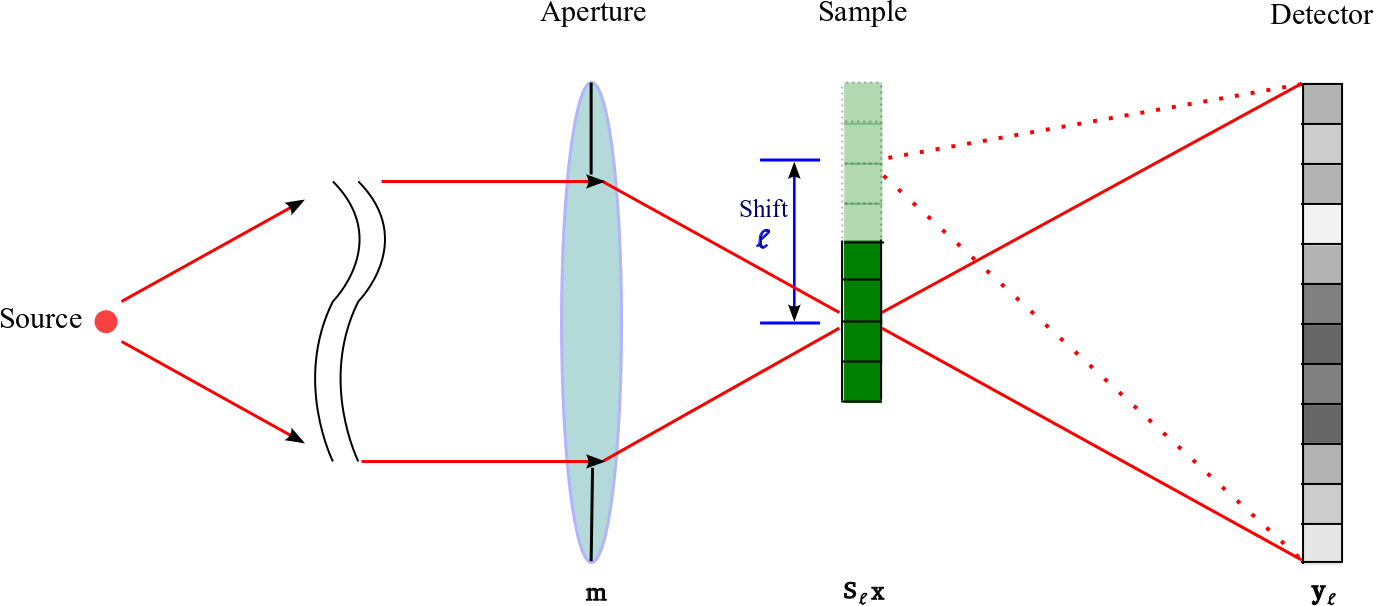
\includegraphics[scale=0.25]{pics/ptych1D}
  \caption[Experimental setup for x-ray crystallography]
          {Experimental setup for x-ray crystallography.   {\small
              (Adapted from ``Fly-scan ptychography'', Huang et al.,
              Scientific Reports 5 (9074), 2015.)}}
  \label{fig:xray_cryst}
\end{figure}

This seemingly simple technique has been indispensable for the study of chemistry, biology, and physics, having been used to confirm or identify the arrangements of atoms in a wide variety of important compounds.  Over a dozen discoveries made through x-ray crystallography -- or made in developing the technique -- have been recognized by Nobel Prizes in Physics, Chemistry, and Medicine or Physiology.  Indeed, the first Nobel Prize in Physics was awarded to Wilhelm R\"ontgen in 1901 for his discovery of x-rays.  The 1914 Prize in Physics was conferred upon Max von Laue for discovering the diffraction of x-rays by atomic crystals, and in 1915 William and Lawrence Bragg earned the same distinction for performing the first complete characterizations of atomic crystal structures \cite{galli2014nobel}.  Since the time of these highly esteemed pioneering discoveries, x-ray crystallography has been used to produce accurate molecular models of a number of drugs (e.g., \cite{cell2001antibios, rasmussen2007adrenergic, schindler2000kinase}), including penicillin in Dorothy Crowfoot Hodgkin's Nobel prize-winning work in 1963 \cite{hodgkin1963penicillin}.  It has elucidated several human biological compounds, including innumerable proteins \cite{kimber2003protein, varsani1993isomerase} and human DNA, for whose analysis in 1953 James Watson, Maurice Wilkins, and Francis Crick were awarded the Nobel prize in 1962, relying on the crystallographic images of Rosalind Franklin \cite{franklin1953nature,watson1962nobel_lecture,watson1953nature,wilkins1953nature}.  And this technology remains extremely relevant today, playing an active role in material sciences, where crystallography is being used to characterize the degradation of lithium-ion batteries \cite{hausbrand2015battery, andrej2018battery} and to study carbon nanostructures such as fullerenes \cite{lamb1990carbon, kroto1985fullerene}, whose analysis earned the 1996 Nobel Prize in Chemistry \cite{galli2014nobel}.

Perhaps the Nobel prizes, among those awarded for developments related to crystallography, most cogent to the present work is that earned by Herbert A.~Hauptman and Jerome Karle in 1985 for their monograph, \emph{Solution of the Phase Problem, I.  The Centrosymmetric Crystal} \cite{hauptman1953monograph}, in which they presented a direct solution to the phase retrieval problem for centrally periodic, discrete functions which are symmetric about the origin (i.e. centrosymmetric crystals).  Even though this was a special case that the literature of the time had focused on quite heavily, Hauptman and Karle's results eclipsed the somewhat heuristic methods put forth by several authors of the time \cite{harker1948phases,sayre1952shannon}, for the simple fact that they provided a clear algorithm with a proof of success on a clearly defined set of problem instances.  This is precisely the class of solutions we attempt to expand in this dissertation.
